\documentclass[final_report.tex]{subfiles}

\begin{document}

\todo{cite ALL images}

\section{Background}

This section focusses on a number of background concepts which will help to gain further understanding of networking practices and protocols which the solution must adhere to. It then gives an overview of the architecture of the Java langugage and explores on some of the key techniques which will be exploited. As this report focusses on performance testing throughout, this section will then cover techniques to test custom programs. It finally looks at related works within the research area and existing frameworks which could be exploited.

\subsection{Network Components}
%http://www.oreilly.com/openbook/linag2/book/ch09.html
%http://etutorials.org/Networking/Check+Point+FireWall/Chapter+10.+Network+Address+Translation/Implementing+NAT+A+Step-by-Step+Example/
%http://computer.howstuffworks.com/nat.htm
%http://www.sans.org/reading-room/whitepapers/vpns/implementing-nat-checkpoint-firewall-1-733
%http://www.erg.abdn.ac.uk/users/gorry/course/inet-pages/arp.html

\todo{intros for background section}

\subsubsection{Models}
\label{sec:models}
%http://www.networksorcery.com/enp/protocol/ip.htm
%http://www.thegeekstuff.com/2012/03/ip-protocol-header/
%http://www.howtogeek.com/169540/what-exactly-is-a-mac-address-used-for/
%http://wiki.openwrt.org/doc/networking/praxis
%http://www.linuxfoundation.org/collaborate/workgroups/networking/kernel_flow
Generally there are 2 well known network models. The Open System Interconnection (OSI) model in Figure \ref{fig:layers} represents an ideal to which all network communication should adhere to while the Transmission Control Protocol/Inter Protocol (TCP/IP) model represents reality in the world. The TCP/IP model combines multiple OSI layers into 1 of its layers simply because not all systems will go through these exact stages depending on the required  application.

\begin{figure}[H]
	\centering
	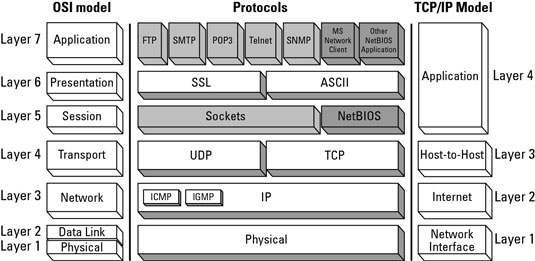
\includegraphics[width=\textwidth]{img/layers.jpg}
	\caption{OSI vs TCP/IP Model}
	\label{fig:layers}
\end{figure}

The TCP/IP application layer doesn't represent an actual application but instead its a set of protocols which provides services to applications. These services include HTTP, FTP, SMTP, POP3 and more. It acts as an interface for software to communicate between systems (e.g. client retrieving data from server via SMTP).

The transport layer is responsible for fragmenting the data into transmission control protocol (TCP) or user datagram protocol (UDP) packets, although other protocols can be used. This layer will attach its own TCP or UDP header to the data which contains information such as source and destination ports, sequence number and acknowledgement data.

The network/internet layer attaches a protocol header for packet addressing and routing. Most commonly this will be an IPv4 or IPv6 header \todo{ref this}. This layer only provides datagram networking functionality and it's up to the transport layer to handle the packets correctly.

The network interface or link layer will firstly attach its own ethernet header (or suitable protocol header) to the packets, along with an ethernet trailer. This header will specify the destination and source of the media access control (MAC) address which are specific to network interfaces. The next step is to put the packet onto the physical layer, which may be fibre optic, wireless or standard cables.

This will eventually build a packet of data which include the original raw data along with multiple headers for each layer of the model (Figure \ref{fig:headers}).

\begin{figure}[H]
	\centering
	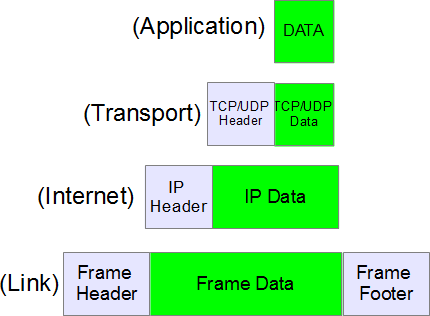
\includegraphics[width=\textwidth]{img/headers.png}
	\caption{Network model building up of data headers}
	\label{fig:headers}
\end{figure}

\subsubsection{Network Packets}
A network packet is responsible for carrying data from a source to a destination. Packets are routed, fragmented and dropped via information stored within the packet's header. Note: in this report packets and datagrams are interchangeable. Data within the packets are generally input from the application layer, and headers are appended to the front of this data depending on the network level described in Section \ref{sec:models}. Packets are routed to their destination based on a combination of an IP address and MAC address which corresponds to a specific computer located within the network, whether that is a public or private network. In this project we will only be concerned with the Internet Protocol (IP) and therefore IPv4 (Figure \ref{fig:ipv4}) and IPv6 (Figure \ref{fig:ipv6}) packet headers.

\begin{figure}[H]
	\centering
	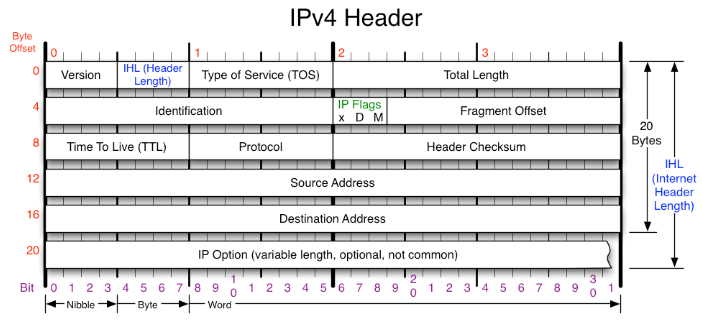
\includegraphics[width=\textwidth]{img/ipv4header.png}
	\caption{IPv4 Packet Header}
	\label{fig:ipv4}
\end{figure}


\begin{itemize}
	\item Version - IP version number (set to 4 for IPv4)
	\item Internet Header Length (IHL) - Specifies the size of the header since a IPv4 header can be of varying length
	\item Type of Service (TOS) - As of RFC 2474 redefined to be differentiated services code point (DSCP) which is used by real time data streaming services like voice over IP (VoIP) and explicit congestion notification (ECN) which allows end-to-end notification of network congestion without dropping packets
	\item Total Length - Defines the entire packet size (header + data) in bytes. Min length is 20 bytes and max length is 65,535 bytes, although datagrams may be fragmented.
	\item Identification - Used for uniquely identifying the group of fragments of a single IP datagram
	\item X Flag - Reserved, must be zero
	\item DF Flag - If set, and fragmentation is required to route the packet, then the packet will be dropped. Usually occurs when packet destination doesn't have enough resources to handle incoming packet.
	\item MF Flag - If packet isn't fragmented, flag is clear. If packet is fragmented and datagram isn't the last fragment of the packet, the flag is set.
	\item Fragment Offset - Specifies the offset of a particular fragment relative to the beginning of the original unfragmented IP datagram
	\item Time To Live (TTL) - Limits the datagrams lifetime specified in seconds. In reality, this is actually the hop count which is decremented each time the datagram is routed. This helps to stop circular routing.
	\item Protocol - Defines the protocol used the data of the datagram
	\item Header Checksum - Used for to check for errors in the header. Router calculates checksum and compares to this value, discarding if they don't match.
	\item Source Address - Sender of the packet
	\item Destination Address - Receiver of the packet
	\item Options - specifies a number of options which are applicable for each datagram. As this project doesn't concern these it won't be discussed further.
\end{itemize}

\begin{figure}[H]
	\centering
	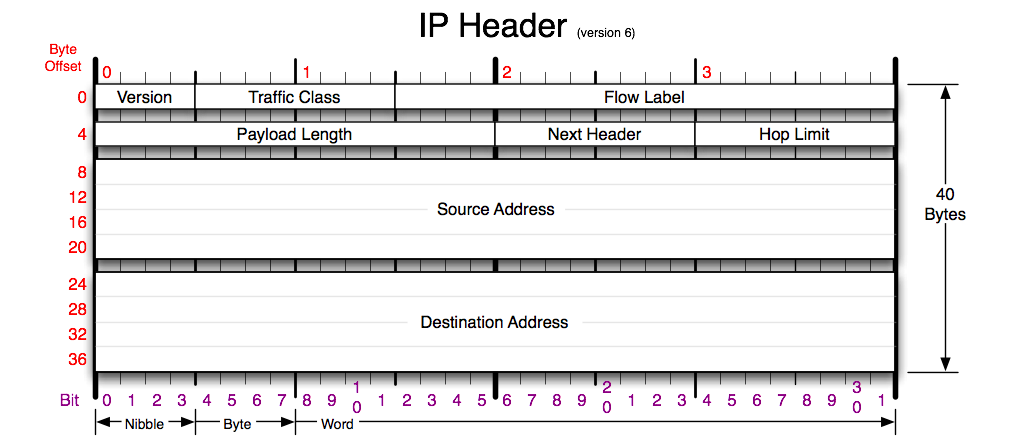
\includegraphics[width=\textwidth]{img/ipv6header.png}
	\caption{IPv6 Packet Header \cite{ipv6}}
	\label{fig:ipv6}
\end{figure}

\begin{itemize}
	\item Version - IP version number (set to 6 for IPv6)
	\item Traffic Class - Used for differentiated services \todo{ref this} to classify packets and ECN as described in IPv4.
	\item Flow Label - Used by real-time applications and when set to a non-zero value, it informs routers and switches that these packets should stay on the same path (if multiple paths are available). This is to ensure the packets arrive at destination in the correct order, although other methods for this are available.
	\item Payload Length - Length of payload following the IPv6 header, including any extension headers. Set to zero when using jumbo payloads for hop-by-hop extensions.
	\item Next Header - Specifies the transport layer protocol used by packet's payload.
	\item Hop Limit - Replacement of TTL from IPv4 and uses a hop value decreased by 1 on every hop. When value reaches 0 the packet is discarded.
	\item Source Address - IPv6 address of sending node
	\item Destination Address - IPv6 address of destination node(s).
	\item Extension Headers - IPv6 allows additional internet layer extension headers to be added after the standard IPv6 header. This is to allow more information for features such as fragmentation, authentication and routing information. The transport layer protocol header will then be addressed by this extension header.
\end{itemize}

\subsubsection{Packet Handling}
\label{subsec:handling}
\todo{is this section right}
Once the kernel of the given operating system has received data to transmit from a given application, the data is then placed into a packet with the correct header and these packets are placed on a IP stack (Figure~\ref{fig:buffer}). Through a few intermediate steps the packets arrive at the driver queue, also known as the transmission queue. This queue is implemented as a ring buffer, therefore has a maximum capacity before it starts to overwrite packets which are still to be transmitted. As long as the queue isn't empty, the network interface card (NIC) will take packets from the queue and place them on the transmission medium. A similar process occurs when receiving packets, but in the opposite direction. For each NIC, there is a receive and transmit queue which are independent of each other allow communication to be bidirectional, although this depends on the kernel and its handling of events associated with packets.

\begin{figure}[H]
	\centering
	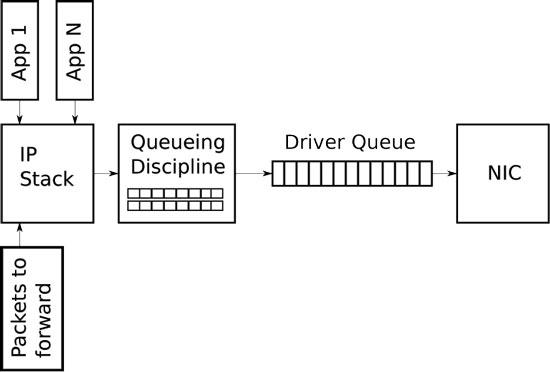
\includegraphics[width=\textwidth]{img/buffer.jpg}
	\caption{Linux packet handling \cite{buffer}}
	\label{fig:buffer}
\end{figure}

\subsubsection{Network Interface Controller (NIC)}
Also known as a Network Interface Card, they provide the ability for a computer to connect to a network through a variety of mediums such as wireless, ethernet and fibre optics. They provide both the data link and physical layer of the network model (Figure \ref{fig:layers}), allowing a protocol stack to communicate with other computers on the local area network (LAN) or over a wider area via the IP protocol using IP addresses.

NICs can run at speeds of up to 100Gbps but more commonly run at 10Gbps for servers and 1Gbps for standard computers. The kernel or other applications retreive packets via the NIC by polling or itterupts. Polling is where the kernel or application will periodically check the NIC for received packets while the use of interupts allows the NIC to tell the kernel or application that it has received packets. Generally NICs provide the ability for 1 or more recieve and transmit queues to be assigned per port, allowing for increased performance by assigning queues to different threads.

\subsubsection{Middleboxes}
Middleboxes are a device within a network that inspect, alter and forwats packers them depending on certain rules and the intended functionaility of the middlebox. A few different types are described below and can be combined into 1 single application:

\paragraph*{Firewall}
Firewalls (Figure~\ref{fig:firewall}) are generally the major applications which sit between the public and private network of a system. They provide packet filtering which controls which packets can enter the private network via establishing a set of rules which packets have to adhere to. Filtering can be based on a number attributes of the packet such as the source and destination IP address and port and the destination service. Firewalls can also offer a number of other useful features such as NAT's or dynamic host configuration protocol (DCHP) to allow dynamic assignment of IP addresses within a network. As well as providing protection on a network level, application layer firewalls exist which stop certain applications from sending or receiving a packet.

\begin{figure}[H]
	\centering
	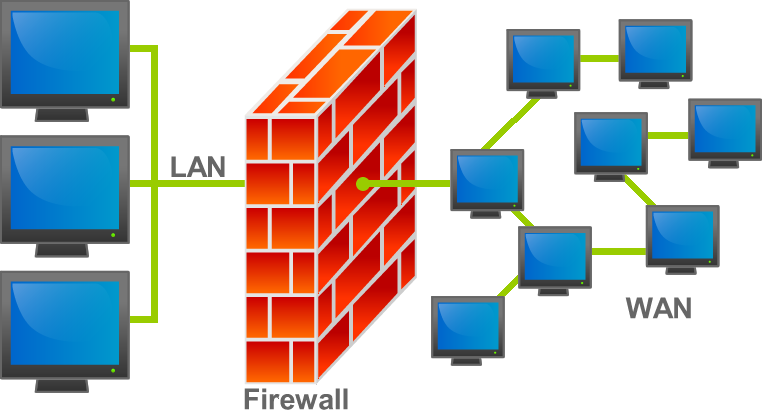
\includegraphics[width=0.7\textwidth]{img/firewall.png}
	\caption{Firewall intercepting packets as a security measure \cite{firewall}}
	\label{fig:firewall}
\end{figure}

\paragraph*{Network Address Translator (NAT)}
\todo{complete this with help from links}
As a routing device, a NAT is responsible for remapping an IP address to another by altering the IP datagram packet header. NAT's have become extremely important in modern networking systems due to IPv4 address exhaustion, allowing a single public IP address to map to multiple private IP addresses. This is particularly useful in large corporations where only a limited public network connection is required, meaning that all private IP addresses (usually associated with a single machine) are mapped to the same public IP address. A NAT will make use of multiple connection ports to identify which packets are for which private IP address and then re-assign the packet header so the internal routers can forward the packet correctly. As can be seen by Table~\ref{tab:ip} and Figure~\ref{fig:nat}, each internal address is mapped to via the port number associated with the external address. NAT's are generally implemented as part of a network firewall as they inspect the datagram packets for malicious data and sources.

\begin{table}[H]
	\centering
	\begin{tabular} { | c | c | }
		\hline
		\textbf{Private IP Address} & \textbf{Public IP Address} \\
		\hline
		10.0.0.1 & 14.1.23.5:62450 \\
		\hline
		10.0.0.2 & 14.1.23.5:62451 \\
		\hline
		10.0.0.3 & 14.1.23.5:62452 \\
		\hline
		10.0.0.4 & 14.1.23.5:62453 \\
		\hline
	\end{tabular}
	\caption{Example of public IP address and ports mapping to private IP address}
	\label{tab:ip}
\end{table}

\begin{figure}[H]
	\centering
	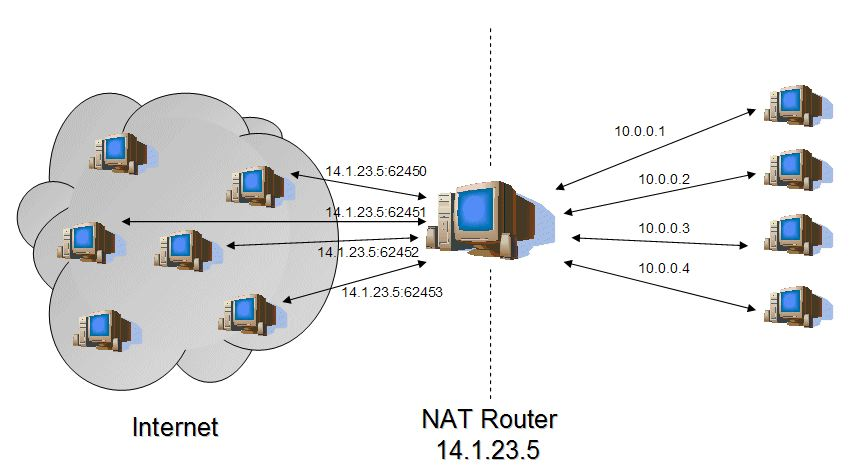
\includegraphics[width=\textwidth]{img/nat.jpg}
	\caption{NAT translating public IP addresses into private IP addresses \cite{nat-table}}
	\label{fig:nat}
\end{figure}

\todo{any more middleboxes - packet cap?}

\subsection{Java}

\subsubsection{JVM}

The Java Virtual Machine is an abstract computer that allows Java programs to run on any computer without dependant compilation. This works by all Java source code been compiled down into Java byte code, which is interpreted by the JVM's just in time (JIT) compiler to machine code. However, it does require each computer to have the Java framework installed which is dependant on the OS and architecture. It provides an appealing coding language due to the vast support, frameworks and code optimisations available such as garbage collections and multithreading. Figure~\ref{fig:jvm} shows the basic JVM architecture with the relevant sections explained in the list below.

\begin{figure}[H]
	\centering
	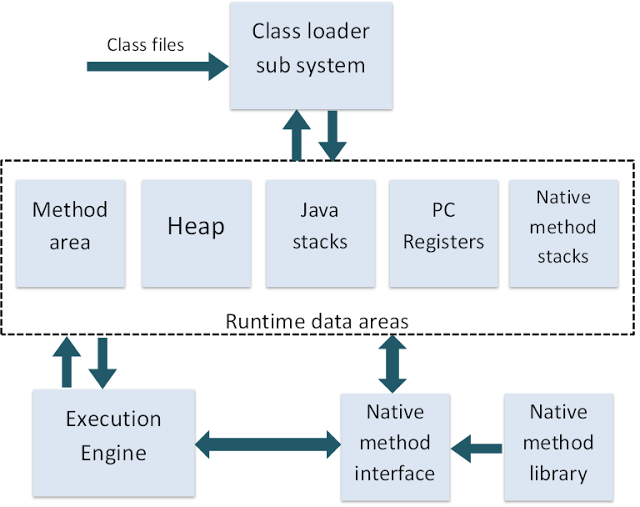
\includegraphics[width=\textwidth]{img/jvm.png}
	\caption{Java Virtual Machine interface \cite{jvm}}
	\label{fig:jvm}
\end{figure}

\begin{itemize}
	\item Class loader sub system - Loads .class files into memory, verifies byte code instructions and allocates memory required for the program
	\item Method area - stores class code and method code
	\item Heap - New objects are created on the heap
	\item Stack - Where the methods are executed and contains frames where each frame executes a separate method
	\item PC registers - Program counter registers store memory address of the instruction to be executed by the micro processor
	\item Native method stack - Where the native methods are executed.
	\item Native method interface - A program that connects the native method libraries with the JVM
	\item Native method library - holds the native libraries information
	\item Execution engine - Contains the interpreter and (JIT) compiler. JVM decides which parts to be interpreted and when to use JIT compiler.
\end{itemize}

Typically, any network communication from a Java application occurs via the JVM and through the operating system. This is because the JVM is still technically an application running on top of the OS and therefore doesn't have any superuser access rights. Any network operation results in a kernel system call, which is then put into a priority queue in order to be executed. This is one of the main reasons why network calls through the JVM and kernel can be seen as 'slow', in relative speeds compared to network line rate speeds.

\subsubsection{Java Native Interface (JNI)}
%http://stackoverflow.com/questions/13973035/what-is-the-quantitative-overhead-of-making-a-jni-call
%http://normanmaurer.me/blog/2014/01/07/JNI-Performance-Welcome-to-the-dark-side/
%http://stackoverflow.com/questions/7823665/why-jni-call-to-native-method-is-slower-than-similar-in-sun-misc-unsafe
%http://stackoverflow.com/questions/7699020/what-makes-jni-calls-slow
%http://stackoverflow.com/questions/17709210/jni-passing-large-amounts-of-data-between-java-and-native-code
%http://docs.oracle.com/javase/1.5.0/docs/guide/jni/spec/types.html#wp16432
%http://www.public.iastate.edu/~java/docs/guide/nativemethod/types.doc.html
%http://journals.ecs.soton.ac.uk/java/tutorial/native1.1/implementing/method.html
%http://docs.oracle.com/javase/1.5.0/docs/guide/jni/spec/types.html
%http://www.ibm.com/developerworks/java/library/j-jni/#reaching
%http://www.mastercorp.free.fr/Ing1/Cours/Java/java_lesson1/doc/Tutorial/performance/JPNativeCode_fm.htm
%http://janet-project.sourceforge.net/papers/jnibench.pdf

Provided by the Java Software Development Kit (SDK), the JNI is a native programming interface that lets Java applications use libraries written in other languages. The JNI also includes the invocation API which allows a JVM to be embedded into native applications. This project and therefore this overview will only focus on Java code using C libraries via the JNI on a linux based system.

In order to call native libraries from Java applications a number of steps have to be undertaken as shown below, which are described in more detail later:

\begin{enumerate}
	\item Java code - load the shared library, declare the native method to be called and call the method
	\item Compile Java code - compile the Java code into bytecode
	\item Create C header file - the C header file will declare the native method signature and is created automatically via a terminal call
	\item Write C code - write the corresponding C source file
	\item Create shared library - create a shared library file (.so) from C code
	\item Run Java program - run the Java program which calls the native code
\end{enumerate}

The Java Framework provides a number of typedef's used to have equivalent data types between Java and C, such as jchar, jint and jfloat, in order to improve portability. For use with objects, classes and arrays, Java also provides others such as jclass, jobject and jarray so interactions with Java specific characteristics can be undertaken from native code run within the JVM.

\begin{lstlisting}[language=Java, caption={Basic Java class showing native method declaration and calling with shared library loading}, label=lst:java]
public class Jni {

	int x = 5;

	public int getX() {
		return x;
	}

	static { System.loadLibrary("jni"); }

	public static native void objectCopy(Jni o);

	public static void main(String args[]) {
		Jni jni = new Jni();
		objectCopy(jni);
	}

}
\end{lstlisting}

Code~\ref{lst:java} shows a simple Java program which uses some native C code from a shared library. Line 9 indicates which shared library to load into the application, which is by default lib*.so where * indicates the name of the library identifier. Line 11 is the native method declaration which specifies the name of the method and the parameters which will be passed to the corresponding C method. In this case, the method name is 'objectCopy' and a 'Jni' object is passed as a parameter. Line 15 is where this native method is called.

\begin{lstlisting}[language=sh, caption={Compiling basic Java program}, label=lst:javacomp]
$ javac Jni.java
\end{lstlisting}

Code~\ref{lst:javacomp}, run from a terminal, compiles the Java class and create a class file which can be executed.

\begin{lstlisting}[language=sh, caption={Generating C header file}, label=lst:gen]
$ javah -jni Jni
\end{lstlisting}

In order to generate the C header file the command 'javah' (Code~\ref{lst:gen}) is used with the flag 'jni' which tells Java that a header file is required which is for use with the JNI. It will then produce method signatures which correspond to the native method declared within Jni.java. The auto generated C header file is shown in Code~\ref{lst:auto}.

\begin{lstlisting}[language=C, caption={Auto-generated C header file}, label=lst:auto]
/* DO NOT EDIT THIS FILE - it is machine generated */
#include <jni.h>
/* Header for class Jni */

#ifndef _Included_Jni
#define _Included_Jni
#ifdef __cplusplus
extern "C" {
#endif
/*
 * Class:     Jni
 * Method:    objectPrint
 * Signature: (LJni;)V
 */
JNIEXPORT void JNICALL Java_Jni_objectPrint
  (JNIEnv *, jclass, jobject);

#ifdef __cplusplus
}
#endif
#endif
\end{lstlisting}

\begin{lstlisting}[language=C, caption={C source file corresponding to auto-generated header file}, label=lst:source]
#include "Jni.h"

JNIEXPORT void JNICALL Java_Jni_objectPrint(JNIEnv *env, jclass class, jobject obj) {
	jclass cls = (*env)->FindClass(env, "Jni");
	jmethodID method = (*env)->GetMethodID(env, cls, "getX", "()I");
	int i = (*env)->CallIntMethod(env, obj, method);
	printf("Object x value is %i\n", i);
}
\end{lstlisting}

The C source file implementation is in Code~\ref{lst:source}. The method signature on line 3 isn't as first declared in the Java source file. The 'env' variable is used to access functions to interact with objects, classes and other Java features. It points to a structure containing all JNI function pointers. Furthermore, the method invocation receives the class from which it was called since it was a static method. If the method had been per instance, this variable would be of type 'jobject'.

Line 4 shows how to find a class identifier by using the class name. In this example, the variables 'class' and 'cls' would actually be equal. In order to call an objects' method, a method id is required as a pointer to this method. Line 5 shows the retrieval of this method id, whose parameters are the jclass variable, the method name and the return type, in this case an integer (represented by an I). Then the method can be called on the object via one of the numerous helper methods (line 6) which differ depending on the return type and static or non-static context.

\begin{lstlisting}[language=sh, caption={Terminal commands to generate shared library file (.so)}, label=lst:shared]
$ gcc -shared -fpic -o libjni.so -I/usr/java/include -I/usr/java/include/linux jni.c
\end{lstlisting}

The command in Code~\ref{lst:shared} will create the shared object file called 'libjni.so' from the source file 'jni.c'. This output file is what the Java program uses to find the native code when called. It requires pointers to the location of the Java Framework provided jni.h header file.

\begin{lstlisting}[language=sh, caption={Output from running Java application calling native C methods}, label=lst:output]
$ java -Djava.library.path="." Jni
Object x value is 5
\end{lstlisting}

Running the Java application, pointing to the location where Java can find the shared library (if not in a standard location) will output the above in Code~\ref{lst:output}.

Although the JNI provides a very useful interface to interact with native library code, there are a number of issues that users should be wary of before progressing:
\begin{itemize}
	\item The Java application that relies on the JNI loses its portability with the JVM as it relies on natively compiled code.
	\item Errors within the native code can potentially crash the JVM, with certain errors been very difficult to reproduce and debug.
	\item Anything instantiated with the native code won't be collected by the garbage collector with the JVM, so freeing memory should be a concern.
	\item If using the JNI on large scale, converting between Java objects and C structs can be difficult and slow
\end{itemize}



\subsubsection{Current Java Networking Methods}
http://haumacher.de/publ/parallel/p086.pdf
http://www.javacoffeebreak.com/articles/javarmi/javarmi.html
For high performance computing in Java, a number of existing programming options are available in order for applications to communicate over a network. These can be classified as: (1) Java sockets; and (2) Remote Method Invocation (RMI); (3) shared memory programming. As will be discussed, none of these are capable of truly high performance networking, especially at line rate speeds.

\paragraph{Java Sockets}\mbox{}\\ %subsubsubsection
\label{subsec:sockets}
Java sockets are the standard low level communication for applications as most networking protocols have socket implementations. They allow for streams of data to be sent between applications as a socket is one end point for a 2 way communication link, meaning that data can be read from and written to a socket in order to transfer data. Even though sockets are a viable option for networking, both of the Java socket implementations (IO sockets \& NIO (new I/O) sockets) are inefficient over high speed networks \cite{sockets} and therefore lack the performance that is required. As discussed previously, the poor performance is due to the JVM interacting with network cards via the OS kernel.

\paragraph{Remote Method Invocation (RMI)}\mbox{}\\ %subsubsubsection
Remote Method Invocation (RMI) is a protocol developed by Java which allows an object running in a JVM to invoke methods on another object running on a different JVM. Although this method provides a relatively easy interface for which JVM's can communicate, its major drawback relates to the speed. Since RMI uses Java sockets as its basic level communication method, it faces the same performance issues as mentioned in section~\ref{subsec:sockets}.

\paragraph{Shared Memory Programming}\mbox{}\\ %subsubsubsection
Shared memory programming provides high performance JVM interaction due to Java's multithread and parallel programming support. This allows different JVM's to communicate via objects within memory which is shared between the JVM's. However, this technique requires the JVM's to be on the same shared memory system, which is a major drawback for distributed systems as scalability options decrease.

Even though these 3 techniques allow for communication between JVM's and other applications, the major issue is that incoming packets are still handled by the kernel and then passed onto the corresponding JVM. This means that packets are destined for certain applications, meaning that generic packets can't be intercepted and checked, which is a requirement for common middlebox software.

\subsection{Related Works}

\subsubsection{jVerbs}
Ultra-low latency for Java applications has been partially solved by the jVerbs \cite{jverbs} framework. Using remote direct memory access (RDMA), jVerbs provides an interface for which Java applications can communicate, mainly useful within large scale data centre applications.

RDMA is a technology that allows computers within a network to transfer data between each other via direct memory operations, without involving the processor, cache or operating system of either communicating computer. RDMA implements a transport protocol directly within the network interface card (NIC), allowing for zero copy networking, which allows a computer to read from another computer and write to its own direct main memory without intermediate copies. High throughput and performance is a feature of RDMA due to the lack of kernel involvement, but the major downside is that it requires specific hardware which supports the RDMA protocol, while also requiring the need for specific computer connections set up by sockets.

As jVerbs takes advantage of mapping the network device directly into the JVM, bypassing both the JVM and operating system (Figure~\ref{fig:jverb}), it can significantly reduce the latency. In order to have low level interaction with the NIC, jVerbs has a very thin layer of JNI calls which can increase the overhead slightly. However, jVerbs is flawed, mainly because it requires specific hardware to run on, firstly limited by the RDMA protocol reliant hardware and further by the required RDMA wrappers which are implemented by the creators. Also, it can only be used for specific computer to computer connection and not generally packet inspection. 

\begin{figure}[H]
	\centering
	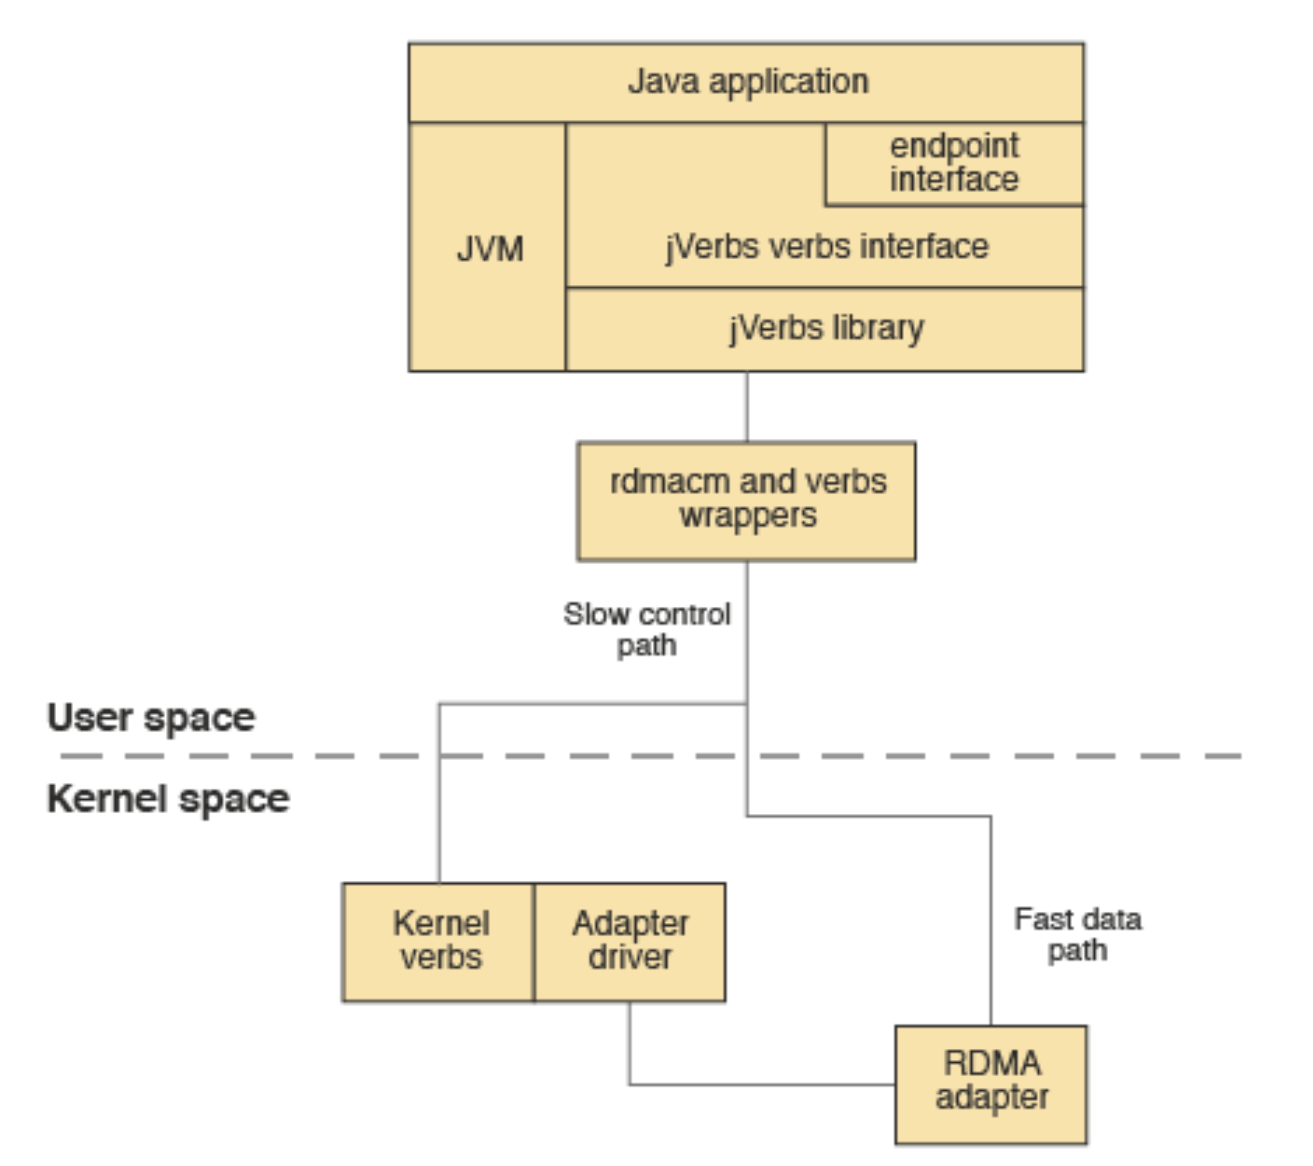
\includegraphics[width=\textwidth]{img/jverbs.png}
	\caption{jVerbs architecture - shows how the framework bypasses the kernel and JVM \cite{ibm_jverbs}}
	\label{fig:jverb}
\end{figure}

jVerbs provides a useful example framework which re-emphasises that packet processing in Java is very possible with low latency, while assisting in certain implementation and design choices which can be analysed in more detail.

\subsubsection{Packet Shader}
The CPU can be a potential bottleneck in high speed software based routers and Packet Shader which aims to eliminate this. It takes advantage of graphic processing units (GPU) which offer greater execution power than typical CPUs due to their ability to run thousands of threads in parallel. By using the GPU and running packet processing threads on the GPU packet shader can increase performance to routers up to 40Gbps. However, the research behind this project has been suspended in favour of DPDK (\ref{subsec:dpdk}).

\subsubsection{Data Plane Development Kit (DPDK)}
\label{subsec:dpdk}
%https://www.youtube.com/watch?v=BqV833_xd-Y
%file:///Users/ashleyhemingway/Downloads/communications-packet-processing-brief.pdf
Data Plane Development Kit (DPDK) \cite{dpdk} is a set of libraries and drivers which enables fast packet processing reaching speeds of 80 million packets per second on certain system set ups. Since DPDK is developed by Intel, it only supports Intel x86 CPU's and certain network interface controllers (NIC). DPDK binds the NIC's to new drivers meaning that the operating system doesn't recognise the network cards and therefore the network stack associated with the ports don't work. It make use of drivers run in user space allowing it to interact with certain memory locations without permission from the kernel or even involving it in any way.

DPDK makes use of an environment abstraction layer (EAL) which hides the environmental specifics and provides a standard interface which any application can interact with. Due to this, if the system changes in any way, the DPDK library needs to be re-compiled with other features been re-enabled in order to allow applications to run correctly again.

In order to use the DPDK libraries for the intended purpose, data packets have to be written into the correct buffer location so they are inserted onto the network. I similar approach is used when receiving packets on the incoming buffer ring, but instead of the system using interrupts to acknowledge the arrival of a new packet, which is performance costly, it constantly polls the buffer space to check for new packets. DPDK also allows for multiple queues per NIC and can handle multiple NIC's per system, therefore scalability is a major bonus of the libraries.

DPDK is very well documented on a number of levels. Firstly there is a online API which gives in depth details about what the methods, constants and structs do. There are a number of well written guides which give step-by-step details of how to install, set-up and use DPDK on various platforms and finally, there are many sample programs included with the build which give understanding of how the overall library works. DPDK is discussed in much more detail in Section \ref{sec:dpdk}.

\subsection{Performance Testing Techniques}
%http://stackoverflow.com/questions/10942985/measuring-overhead-of-calling-through-jni
%https://code.google.com/p/multi-language-bench/source/checkout
%https://days2011.scala-lang.org/sites/days2011/files/ws3-1-Hundt.pdf
%http://www.jeremyong.com/blog/2013/08/29/stop-comparing-programming-languages-with-benchmarks/
%https://attractivechaos.github.io/plb/
%http://economics.sas.upenn.edu/~jesusfv/comparison_languages.pdf
Benchmarking is a process of testing hardware, individual components or full end to end systems to determine the performance of the application or hardware \todo{Examples of hardware comparisons}. Generally, benchmarking should be repeatable under numerous iterations without only minor variations in performance results. This is firstly to allow minor changes to be made to the application/component with re-runs of the benchmark showing the performance changes. Secondly, it allows accurate comparisons to be drawn between similar software or hardware with different implementations in order to derive \todo{better word for derive} a better product.

\todo{why I need benchmarking}

\subsubsection{Programming Languages}
It is well known that different programming languages can provide a radical change in execution for a given program. However, direct comparisons can't truly be trusted as certain languages are suited for for specific tasks and finding a benchmarking program to incorporate this is problematic. Other factors can be introduced when deciding on the optimisation level \todo{show example of optimising java and how different it looks, also different depending on architecture} and the compiler of JIT used. \todo{better phrasing off that sentence needed}

Numerous attempts have been made to compare languages, most noticeably the 'Benchmark Game' and Google. \todo{More here}
\paragraph{Loop Recognition}\mbox{}\\
Google inducted their own experiment on this problem, testing only C++, Java, Scala and Go on the loop recognition algorithm \todo{get paper}. Implementations made use of standard looping constructs and memory allocation schemes without the use of non-orthodox optimisation techniques. Selected results of this are shown below: \todo{explain difference with GC etc}

\begin{table}[H]
	\centering
	\begin{tabular} { | c | c | c | }
		\hline
		\textbf{Benchmark} & \textbf{Time [sec]} & \textbf{Facter} \\
		\hline
		c++ & 23 & 1.0x \\
		\hline
		Java 64-bit & 134 & 5.8x \\
		\hline
		Java 32-bit & 290 & 12.8x \\
		\hline
		Java 32-bit GC & 106 & 4.6x \\ 
		\hline
		Scala & 82 & 3.6x \\ 
		\hline
		Go 6g & 161 & 7.0x \\
		\hline
	\end{tabular}
	\caption{Results from Loop Recognition benchmarking}
	\label{tab:loop_recog}
\end{table}

\paragraph{Benchmark Game}\mbox{}\\
The Benchmark Game is an online community which aims to find the best programming language by using multiple benchmarking algorithms running on different architecture configurations to determine the outcome. Again, even this community regard the best benchmark application to be your application. A few selected results are shown below between Java and C (those used in this report) for a few different benchmarks. \todo{get data}

\paragraph{Using Economics}\mbox{}\\
About economics paper

\paragraph{Which is better?}

\subsubsection{Intra-Language Techniques}
\subsubsection{Applications}

\end{document}